\graphicspath{{members/cm/figures/}}

\subsection{Building the foundation of the tomato plants}
\input{members/cm/authors}

The goal of the simulation is to create a variety of different realistic tomato plants. The first step is therefore to determine which parameters describe a realistic tomato plant and in what ways they can vary. A tomato plant can be divided into four major parts; stem, leaves, flowers, fruits. Each of which, has its own properties, which can vary from plant to plant in a fixed range. For example, when we are thinking of a tomato plant, we are picturing round, red fruits. But in reality the fruits can vary in size and color depending on the health status of the plant and growth status of the fruit. 

In order to create this variability PlantStudio is used, which is a parameter-driven simulation tool, that can be used for the simulation of various non-woody plants throughout their life cycle. It provides various parameters concerning the structure and the growth of the plant. It starts with a collection of questions regarding the optics of the plant, containing information about the previously named parts of tomato plants. To specify the positioning of fruits and flowers the inflorescence is added to the parameters, which is the part of the plant that holds the fruits and flowers. The stem is described inform of the meristems and internodes. A detailed description of the individual plant parts considered in PlantStudio and how they were set to create the tomato plants can be found in table \ref{tab:parameters_plantStudio}. These parameters enable an individual adjustment of color, shape, amount and distribution for each of these plant parts. Thanks to the randomize function provided by PlantStudio a multitude of different plants with these parameters can be created. Since there is no API for PlantStudio available we had to create the randomized plants manually instead of using an script. For this reason we decided that a total of 42 plants would be enough for the basis of the simulation. \\

For each created plant PlantStudio animates a life cycle going from the spearing of the plant to the full-grown tomato plant with ripe fruits. The duration of the life cycle and at which point the fruits start to grow, can be manually adjusted to create a realistic representation. \\

\begin{longtable}[c]{@{}p{0.15\textwidth}p{0.45\textwidth}p{0.4\textwidth}@{}}
	\caption{General parameters in PlantStudio and how they were set to describe the general appearance of tomato plants.}
	\label{tab:parameters_plantStudio}\\
	\toprule
	& Description                                                                                                                                                                                                                 & Settings                                                                                                                                                                      \\* \midrule
	\endhead
	%
	\bottomrule
	\endfoot
	%
	\endlastfoot
	%
	Meristems               & Meristems are buds from which leaves and branches grow.                                                                                                                                                                     & \vspace{-25pt}
	 \begin{itemize}
		\item opposing to each other \vspace{-10pt}
		\item medium amount of branches \vspace{-10pt}
		\item secondary branches \vspace{-10pt}
		\item angle stem/branch: medium \vspace{-10pt}   
	\end{itemize} \\
	Internodes              & Internodes are portions of plant stem between leaves and determine how short or tall, straight or viney, and stiff or flexible the plant will be                                                                            & \vspace{-25pt}
	\begin{itemize}
		\item long \vspace{-10pt}
		\item medium thickness \vspace{-10pt}
		\item introduce some curve to the plant \vspace{-10pt}
	\end{itemize} \\
	Leaves                  & Leaves are drawn using a 3D-object. The leaf is drawn bigger as the plant grows. Leaves are connected to the plant by a stalk called petiole& \vspace{-25pt}
	\begin{itemize}
		\item pre-build shape: tomato leaf\vspace{-10pt}
		\item small size \vspace{-10pt}
		\item petiole of medium length \vspace{-10pt}
		\item angle stem/leaf: large \vspace{-10pt}
	\end{itemize} \\
	Compound leaves         & A compound leaf contains $>$=2 leaflets. Leaflets look like small whole leaves, but fit together in the same pattern for all leaves of the plant. A leaf without leaflets is a simple leaf & \vspace{-25pt}
	\begin{itemize}
		\item pinnate leaves (seven leaves are ordered feather like) \vspace{-10pt}
		\item leaflet are in a medium distance to each other \vspace{-10pt}
	\end{itemize} \\
	Inflorescence placement & An inflorescence holds fruits and flowers on a plant. It is divided in apical, which means at the end of the plant stems and axillar, which means between the angles between the stem and the leaf.         & \vspace{-25pt}
	\begin{itemize}
		\item no apical inflorescence \vspace{-10pt}
		\item multiple axillary inforescneces (10)\vspace{-10pt}
		\item primary stems have a medium length\vspace{-10pt}
	\end{itemize} \\
	Inflorescence drawing   & Inflorescence can have a variety of shapes                                                                                                                                                                                  & \vspace{-25pt}
	\begin{itemize}
		\item 10 flowers per inflorescence\vspace{-10pt}
		\item placed in spikes\vspace{-10pt}
		\item stem thickness:  medium\vspace{-10pt}
	\end{itemize} \\
	Flowers                 & Like leaves flowers are drawn as 3D objects, with each 3D object representing one petal of the flower.                                                                                                                      & \vspace{-25pt}
	\begin{itemize}
		\item 4 small, yellow pedals\vspace{-10pt}
		\item pre-built shape: corn leaves\vspace{-10pt}
		\item elongated and pointy\vspace{-10pt}
	\end{itemize} \\
	Fruits   & Fruits are drawn like flowers, but with a portion of fruit rotated around instead of petals                                                                                                                                 & \vspace{-25pt}
	\begin{itemize}
		\item common fruit section 1\vspace{-10pt}
		\item 10 fruit sections per fruit\vspace{-10pt}
		\item huge size\vspace{-10pt}
		\item unripe fruits: green\vspace{-10pt}
		\item ripe fruits: red\vspace{-10pt}
	\end{itemize}
\\* \bottomrule
\end{longtable}
\pagebreak

\begin{figure}[ht]
	\centering
	\begin{subfigure}{.24\textwidth}
		\centering
		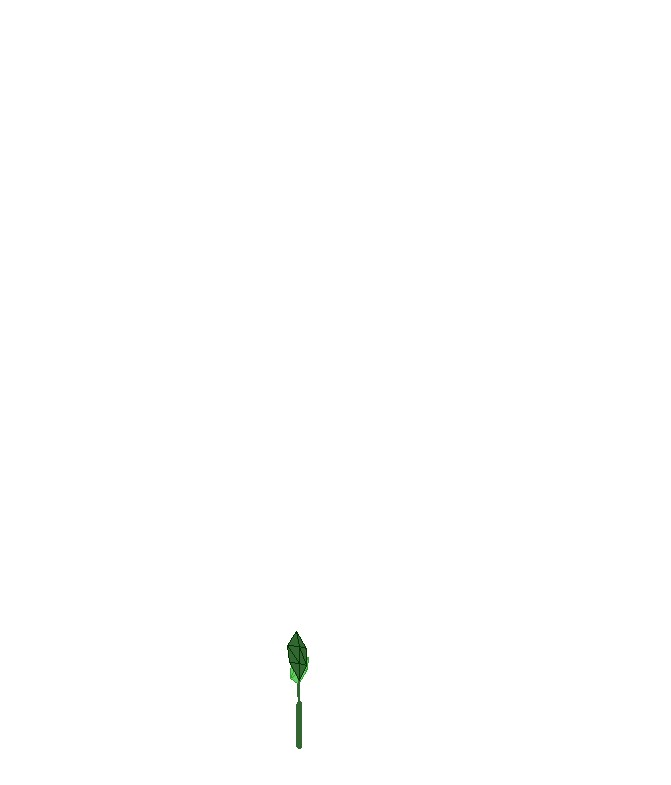
\includegraphics[width=\linewidth]{plantAging001.jpg}
		\label{fig:sub1}
	\end{subfigure}
	\begin{subfigure}{.24\textwidth}
		\centering
		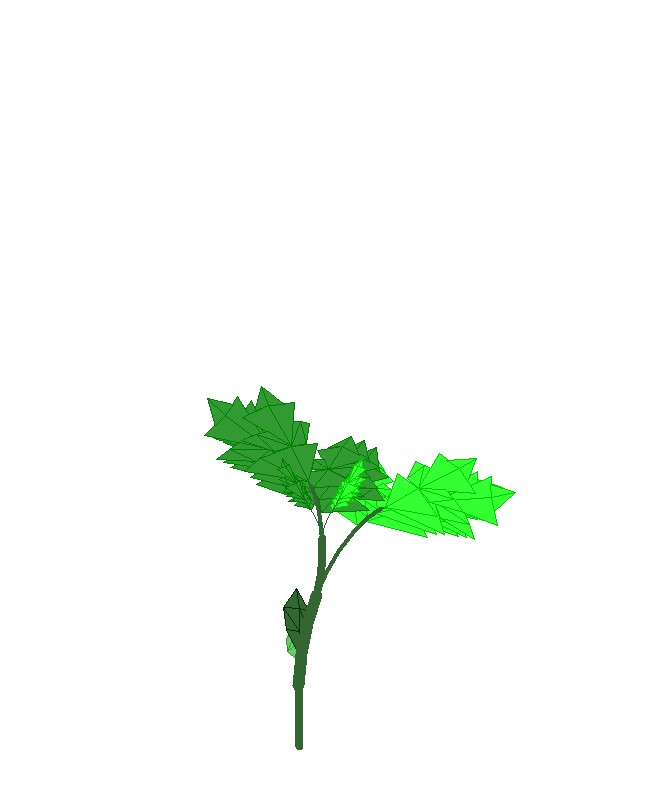
\includegraphics[width=\linewidth]{plantAging002.jpg}
		\label{fig:sub2}
	\end{subfigure}%
	\begin{subfigure}{.24\textwidth}
		\centering
		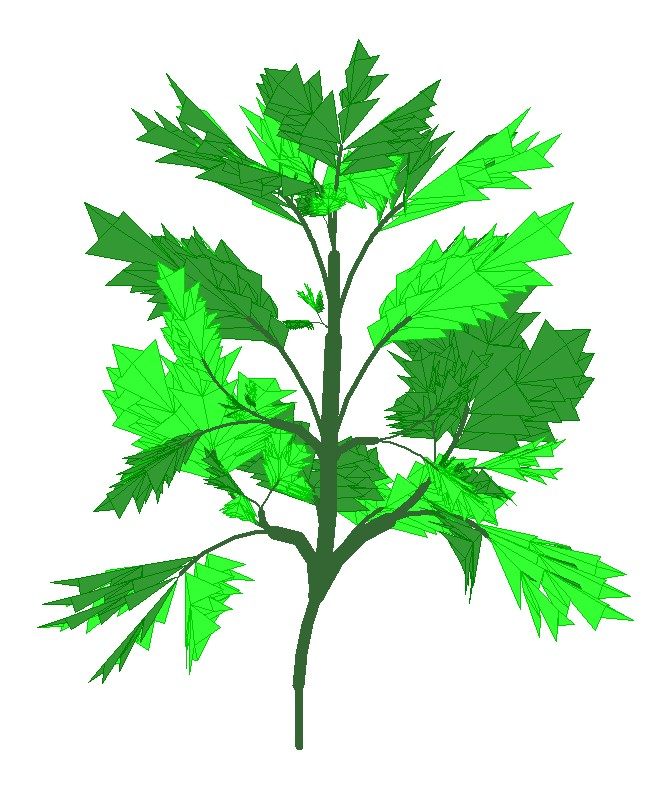
\includegraphics[width=\linewidth]{plantAging003.jpg}
		\label{fig:sub3}
	\end{subfigure}%
	\begin{subfigure}{.24\textwidth}
		\centering
		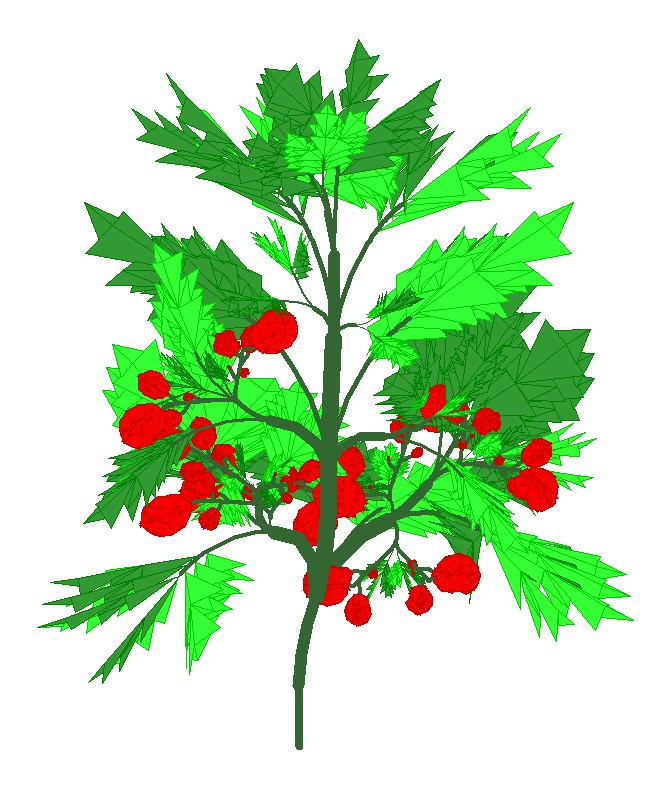
\includegraphics[width=\linewidth]{plantAging004.jpg}
		\label{fig:sub4}
	\end{subfigure}%
	\caption{Exemplary representation of a tomato plant created with the parameters described in table \ref{tab:parameters_plantStudio} in four stages of its life cycle. Showing the growth behavior of the plant going from seedling to a full grown plant with ripe fruits.}
	\label{fig:plantStudio}
	\vspace{-10pt}
\end{figure} 


The created plants have the general parameters of tomato plant but do not look realistic thus far, which can be seen in figure \ref{fig:plantStudio}. The shortcomings of the simulation, like the missing texture and material, can be solved by using a second simulation tool, like Blender. This is enabled by PlantStuios option to export the plants as wavefronts (.obj). PlantStudio provides multiple settings to group the plant when exporting it; whole plant, type of plant part and individual plant part. Since we need the possibility to change single parts of the plant without effecting the rest of the plant, we exported the plants grouped by individual plant parts. The name of each individual plant part contains the type of the plant type, which means that all elements of one type can be found with a simple string matching later. It is also possible to export multiple plants in one file, but this would hinder us in placing them individually in Blender. For this reason we decided to save each of the 42 plants in an own file. These files are saved in one folder, which will be used as input for Blender. \\

The general parameters of tomato plants can vary depending on the type of tomato looked at and on what the focus of the modeling lies. If the requirements of the model would change in later steps of the project, the parameters set in PlantStudio could be updated and the following scripts could without further adjustment be run for the new plants. This empowers a continuously changing simulation, that can grow hand in hand with the model. For a continuing project it would be interesting to write a script that automatically exports a multitude of randomized plants form PlantStudio, as it would further improve the flexibility of the simulation and with it the ability to react to changes in the requirements given by the model.


\subsection{Importing and placing plants in Blender}
\input{members/cm/authors}


The from PlantStudio exported plants can be imported into Blender for further simulation steps. Blender is an open source computer graphics software, which can be used for visual effects, 3D models, etc. The purpose of using Blender is to import the in PlantStudio created plants and  add details, shading, materials, textures, rendering and lighting. 

\begin{wrapfigure}{r}{0.55\textwidth} 
	\vspace{-15pt}
	\begin{center}
		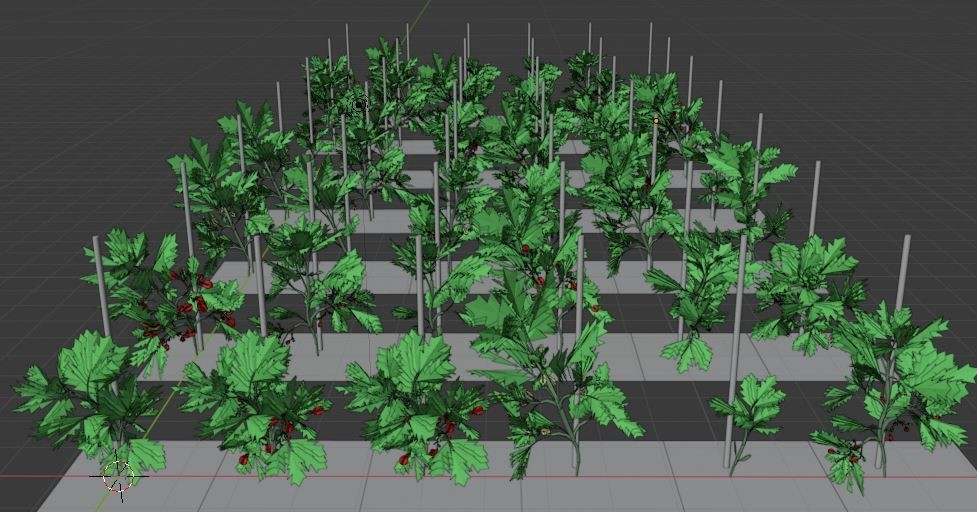
\includegraphics[width=0.55\textwidth]{BlenderImport.JPG}
		\caption{Import of 42 randomly selected plants into Blender with 6 plants per row and soil and pole for each plant.}
		\label{fig:BlenderImport}
	\end{center}
	\vspace{-20pt}
\end{wrapfigure} 

The script written to import the plants can be easily adjusted in the number of plants that should be planted and the number of plants that are placed in each row. These parameters can be set according to what is required. For the current model it is only imported that the photographed plants have neighboring plants on all sides to simulate the noise in the pictures.\\

Which plants are planted is randomly selected from the 42 plants exported from PlantStudio. The folder with the tomato plants can easily be changed or extended if the simulation would be updated. To import a plant it is necessary that the wavefront file is in the given folder and that the file ending is .obj. 

\lstinputlisting[language=Python, linerange={12-14}, frame=single, caption =nrPlants plants are randomly selected from folder \textit{directory\_im} holding obj files ]{members/cm/import_plants.py}\vspace{5pt}

\lstinputlisting[language=Python, linerange={21-39}, frame=single, caption = Inorder to place the plants like they would be placed in the greenhouse we need to know how many plants should be planted and how many fit in one row.]{members/cm/import_plants.py}\vspace{5pt}

In the next step the plants are imported and placed in multiple rows of a specific length, that can be set by the user. Here, it is important to select to split the geometry by group, in order to make the individual adjustment of each leaf or fruit section possible. In the interest of enabling the differentiation of various plants, each plant is saved in its own collection. 

Each plant is positioned next to a pole to fix it and on a square of soil. In this step we add these features without any texture and material. These will be added at a later point to further increase the closeness to reality. 

\lstinputlisting[language=Python, linerange={43-49}, frame=single, caption = Placement of the pole next to each plant. Placement of soil is don analog]{members/cm/import_plants.py}\vspace{5pt}

Further changes in the greenhouse set up introduced by the used model or the user, could be added to this script, again without effecting previous of following steps. This modularity again increases the flexibility and reactivity of the simulation, which is needed for a big project since the model would be always improving and therefore the requirements might change, as well. 